%%%%%%%%%%%%%%%%%%%%%%%%%%%%%%%%%%%%%%%%%
% eBook 
% LaTeX Template
% Version 1.0 (29/12/14)
%
% This template has been downloaded from:
% http://www.LaTeXTemplates.com
%
% Original author:
% Luis Cobo (luiscobogutierrez@gmail.com) with extensive modifications by:
% Vel (vel@latextemplates.com)
%
% License:
% CC BY-NC-SA 3.0 (http://creativecommons.org/licenses/by-nc-sa/3.0/)
%
%%%%%%%%%%%%%%%%%%%%%%%%%%%%%%%%%%%%%%%%%

%----------------------------------------------------------------------------------------
%	DOCUMENT CONFIGURATIONS AND INFORMATION
%----------------------------------------------------------------------------------------

\documentclass[14pt]{memoir} % Font size



%----------------------------------------------------------------------------------------
%	GRAYSCALE EM TODAS AS FIGURAS
% Habilita o modo impressão em tons de cinza, não todo logicmente
% Mas a maioria das coisas, as figuras não, isto é para mandar à editora em GRAY SCALE
%----------------------------------------------------------------------------------------

%%% \def\EnableGrayScale{1}

%----------------------------------------------------------------------------------------
%	Muda La direccion raiz
%----------------------------------------------------------------------------------------
\def \SourceRootPath{.}


%----------------------------------------------------------------------------------------
%	DATOS DEL LIBRO
%----------------------------------------------------------------------------------------
\newcommand{\mytitle}[0]{Aulicha}
\newcommand{\mysubtitle}[0]{Cr{\^o}nicas nos andes}
\newcommand{\myauthor}[0]{Fernando Pujaico Rivera}
\newcommand{\imprimiredition}{Primeira Edi\c{c}\~{a}o} % Book edition
%%% las aventuras de aulicha -crónicas en los andes (Mariano Pujaico Rivera)
%----------------------------------------------------------------------------------------

%----------------------------------------------------------------------------------------
%   Tamanho da folha
%----------------------------------------------------------------------------------------
\def \imprimirpagewidthcm{14.8}  %% A5 
\def \imprimirpageheightcm{21.0} %% A5
%% \def \imprimirpagewidthcm{21.0}  %% A4 
%% \def \imprimirpageheightcm{29.7} %% A4


%----------------------------------------------------------------------------------------
%   DADOS ficha catalográfica
%----------------------------------------------------------------------------------------
\def \myauthorname{Fernando}
\def \myauthorlastname{Pujaico Rivera}
\def \myauthorborn{1982}
\def \imprimirlocal{Lavras}%cidade obrigatorio
\def \imprimiryear{2020}
\newcommand{\imprimirdata}[0]{agosto de \imprimiryear}
\def \imprimirtipotrabalho{Inclui Bibliografia}
\def \imprimirISNI{\href{http://isni.org/isni/000000049156373X}{0000 0004 9156 373X}}
\def \imprimirOrcid{\url{https://orcid.org/0000-0002-4970-2818}}
\def \imprimircuttersanborn{\textcolor{red}{P979X}} %% Nome+titulo %% https://www.cuttersonline.com/app/generator/?q=Pujaico&ref=sanborn&add=
\newcommand{\imprimirpapersize}[0]{{\imprimirpagewidthcm}x{\imprimirpageheightcm}cm}%%{21x30cm}
\def \imprimirCDD{028.5}        %% 028.5 - conto infantil                  %% https://books.google.com.br/books?id=G2xHIl0suOcC&pg=PP46&dq=conto+infantil+cdd&hl=pt-BR&sa=X&ved=2ahUKEwiVq_un6ZnrAhWgILkGHSBeCQkQ6AEwBHoECAEQAg#v=onepage&q=conto%20infantil%20cdd&f=false
                                                                           %% https://books.google.com.br/books?id=bAxcCgAAQBAJ&pg=PA2&dq=conto+infantil+cdd&hl=pt-BR&sa=X&ved=2ahUKEwiVq_un6ZnrAhWgILkGHSBeCQkQ6AEwAnoECAUQAg#v=onepage&q=conto%20infantil%20cdd&f=false
                                %% 808 - Coleções de Literatura e Retórica %% http://bilica.org.br/sistema/modulos/acervo/cdd.php?codigo=800#800
                                %% 808.899282 - LITERATURA INFANTIL        %% http://www.biblivre.org.br/forum/viewtopic.php?f=87&t=3097
                                                                           %% https://www.oclc.org/content/dam/oclc/dewey/updates/ddc23/808.8Manual_20130329_DDC%2023.pdf
                                %% 898 - Nativas das América do Sul        %% http://bilica.org.br/sistema/modulos/acervo/cdd.php?codigo=890#800
\def \imprimirCDU{087.5}        %% Publicações para jovens e infantis      %% https://bibliotextos.files.wordpress.com/2014/07/cdu-parte-i.pdf
\newcommand{\imprimirisbn}[0]{\textcolor{red}{XXX-XX-XX-XXXXX-X}}
\def \imprimireditora{Edi\c{c}\~{a}o Independente}%%{Autopublica\c{c}\~{a}o}%%{Edi\c{c}\~{a}o Independente}
\def \palavraschavea{Conto infantil}
\def \palavraschaveb{Conto peruano}
\def \palavraschavec{Literatura Latino-Americana}
\def \palavraschavesInglesa{children's tale}
\def \palavraschavesInglesb{Peruvian tale}
\def \palavraschavesInglesc{Latin American Literature}
%----------------------------------------------------------------------------------------


%----------------------------------------------------------------------------------------
%	XCOLOR
%----------------------------------------------------------------------------------------
\usepackage[dvipsnames*,svgnames]{xcolor}

\definecolor{colorlowgray}{RGB}{240,240,240}

%----------------------------------------------------------------------------------------
%	COLOR
%----------------------------------------------------------------------------------------
\usepackage{color}

%----------------------------------------------------------------------------------------

%----------------------------------------------------------------------------------------
%----------------------------------------------------------------------------------------
%----------------------------------------------------------------------------------------
\input{\SourceRootPath/structure} % el estilo visual do livro

%----------------------------------------------------------------------------------------
%  footnote font size
%----------------------------------------------------------------------------------------
\renewcommand{\footnotesize}{\small}

%----------------------------------------------------------------------------------------
%	Horizontal separator line
%   \HRule{2pt}
%----------------------------------------------------------------------------------------
\newcommand{\HRule}[1]{\rule{\linewidth}{#1}} % creo el comando  \HRule regla horizontal



%----------------------------------------------------------------------------------------
%	Horizontal separator line
%   \PRLsep{Text}
%----------------------------------------------------------------------------------------
\newlength{\PRLlen}
\newcommand*\PRLsep[1]{\settowidth{\PRLlen}{#1}\advance\PRLlen by -\textwidth\divide\PRLlen by -2\noindent\makebox[\the\PRLlen]{\resizebox{\the\PRLlen}{1pt}{$\blacktriangleleft$}}\raisebox{-.5ex}{\textbf{#1}}\makebox[\the\PRLlen]{\resizebox{\the\PRLlen}{1pt}{$\blacktriangleright$}}\bigskip}


%----------------------------------------------------------------------------------------
%----------------------------------------------------------------------------------------
%----------------------------------------------------------------------------------------
%----------------------------------------------------------------------------------------
% BOX - TCOLORBOX
%----------------------------------------------------------------------------------------
\usepackage[most,many]{tcolorbox}
\usetikzlibrary{decorations.pathmorphing}
\tcbuselibrary{skins}


%%%%%%%%%%%%%%%%%%%%%%%%%%%%%%%%%%%%%%%%%%%%%%%%%%%%%%%%%%%%%%%%%%%%%%%%%%%%%%%%
%%%%%%%%%%%%%%%%%%%%%%%%%%%%%%%%%%%%%%%%%%%%%%%%%%%%%%%%%%%%%%%%%%%%%%%%%%%%%%%%
%%%%%%%%%%%%%%%%%%%%%%%%%%%%%%%%%%%%%%%%%%%%%%%%%%%%%%%%%%%%%%%%%%%%%%%%%%%%%%%%
%%%%%%%%%%%%%%%%%%%%%%%%%%%%%%%%%%%%%%%%%%%%%%%%%%%%%%%%%%%%%%%%%%%%%%%%%%%%%%%%
%% UN SOLO USO
%%%%%%%%%%%%%%%%%%%%%%%%%%%%%%%%%%%%%%%%%%%%%%%%%%%%%%%%%%%%%%%%%%%%%%%%%%%%%%%%


%----------------------------------------------------------------------------------------
% CATALOGRAFICA MESSAGE BOX
%----------------------------------------------------------------------------------------
% \begin{catalografica}
%   texto
% \end{catalografica}

\newtcolorbox{catalografica}
{
  breakable,
  enhanced,
  arc=0mm,
  width=\textwidth,
  colback  = white,
  colframe = black
}

 % las macros compuestas usadas para la escrita
%----------------------------------------------------------------------------------------

\hyphenation{zan-dor}
\hyphenation{zo-rra}
\hyphenation{A-ya-cu-cho}

%-----------------------------------------------------------------------------------------
% evitar linhas órfãs e viúvas
%\clubpenalty=100000 
%\widowpenalty=100000 
%-----------------------------------------------------------------------------------------

%----------------------------------------------------------------------------------------
% Agrega marca de agua a cada pagina do livro
%----------------------------------------------------------------------------------------
\begin{comment}
\usepackage{draftwatermark}
\SetWatermarkText{Preview-Preview}
\SetWatermarkColor[gray]{0.9}
\SetWatermarkScale{1}
\end{comment}
%-----------------------------------------------------------------------------------------

\title{\mytitle} % Book title
\author{\myauthor} % Author


%----------------------------------------------------------------------------------------
%	My macros
%----------------------------------------------------------------------------------------
\makeatletter
\newcommand{\showfont}{codifica\c{c}\~ao: \f@encoding{},
  familia: \f@family{},
  serie: \f@series{},
  %shape: \f@shape{},
  e tamanho: \f@size{} pt
}



\newcommand{\AulichaEdad}{10}
\newcommand{\AulichaAnho}{1930} 


%----------------------------------------------------------------------------------------

\begin{document}

\frontmatter
%----------------------------------------------------------------------------------------
%	TITLE PAGE
%----------------------------------------------------------------------------------------
\cleardoublepage
\newpage
\thispagestyle{empty}

\ThisCenterWallPaper{1.00}{background2.eps} % Add the background image, the first argument is the scaling - adjust this as necessary so the image fits the entire page
%\ThisULCornerWallPaper{1.0}{background2}

%% \begin{comment}
\begin{titlepage}
\begin{center}
%% Upper part of the page
%\includegraphics[width=1\textwidth]{./up-logo.jpg}\\[0.4cm]    
\textsc{\LARGE Primeira Edição}\\[0.25cm]
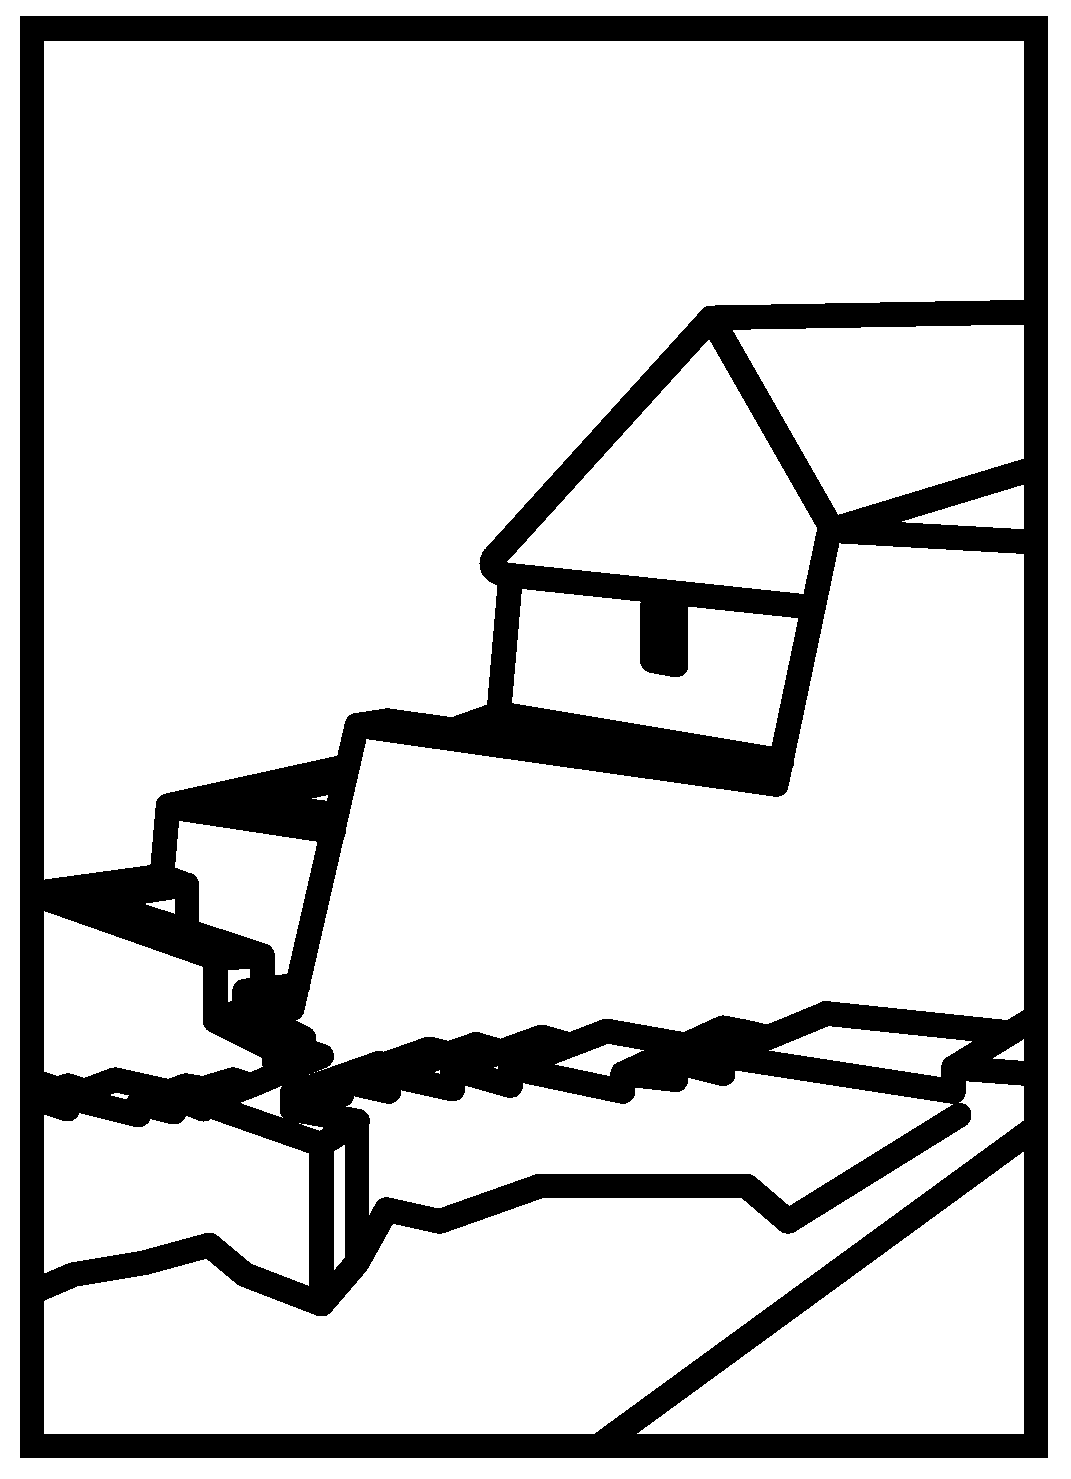
\includegraphics[width=0.25\textwidth]{principal}\\[0.25cm]
%% Title
%\HRule{0.4cm} \\[0.4cm]
\includegraphics[width=0.92\textwidth]{bar}\\[0.2cm]
{ \huge \bfseries \mytitle}\\[0.4cm]
%\HRule{0.4cm} \\[0.7cm]
\includegraphics[width=0.92\textwidth]{bar}\\[0.4cm]
%% SubTitle
{\LARGE \textsc{\mysubtitle}}\\[0.5cm]
\vfill
%% Author 
\textsc{\Large  \myauthor }
\vfill
\textsc{\Large Lavras/MG}\\[0.4cm]
\textsc{\Large \imprimiryear}
\end{center}
\end{titlepage}
%% \end{comment}


%----------------------------------------------------------------------------------------
%	COPYRIGHT PAGE
%----------------------------------------------------------------------------------------
%\cleardoublepage

\newpage
\thispagestyle{empty}

{\small

\noindent Copyright \copyright\ \imprimiryear\ \myauthor\\ % Copyright notice
\noindent \textbf{ISNI  ::} \imprimirISNI\\
\noindent \textbf{ORCID ::} \imprimirOrcid\\
~\\
\noindent \textbf{Impresso no Brasil -- ISBN:} \imprimirisbn\\ % Publisher
\noindent \textbf{Publicado:} \imprimireditora\\ % Publisher
\noindent \textbf{Primeira impressão:} \imprimiryear\\ % Printing/edition date
\noindent \textbf{Diagramação:} \myauthor\\ % Printing/edition date
\noindent \textbf{Revisão de texto:} \textcolor{red}{XXXXXX XXXXXX}\\ % Printing/edition date
\noindent \textbf{Capa:} \myauthor\\ % Printing/edition date
~\\
\textbf{Ficha catalográfica}
\begin{center}
\begin{catalografica}%%
	\myauthorlastname, \myauthorname, \myauthorborn.%Sobrenome, Nome do autor

	\hspace{0.5cm} \mytitle: \mysubtitle~/ \myauthor. -- %\mytitle inicia na quarta letra do sobrenome
	\imprimirlocal, \imprimireditora, \imprimiryear.
	
	\hspace{0.5cm} \pageref{LastPage} p.: \imprimirpapersize.\\ %: il. (algumas color.) ; \imprimirpapersize.
	
	\hspace{0.5cm}
	\parbox[t]{\textwidth}{\imprimirtipotrabalho}%~--~\imprimireditora,~\imprimirdata.}\\

	\hspace{0.5cm}
	\parbox[t]{\textwidth}{ISBN: \imprimirisbn}\\


	\hspace{0.5cm}
	\begin{inparaenum}[1.]
		\item \palavraschavea.
		\item \palavraschaveb.
		\item \palavraschavec.
	\end{inparaenum}
	\begin{inparaenum}[I.]
		\item Título.% O livro deve ser encontrado pelo titulo
	\end{inparaenum}

    \begin{flushright}
    CDD: \imprimirCDD\\
    CDU: \imprimirCDU
    \end{flushright}
\end{catalografica}%%
\end{center}

}


%----------------------------------------------------------------------------------------
%	DEDICATORIA
%----------------------------------------------------------------------------------------
%\cleardoublepage

\null
\vfill
\thispagestyle{empty}



{\normalsize \it \hfill Dedico este livro 
a meu pai Aurelio Pujaico Osccorima, 
a minha mãe Flaviana Rivera Illanes
e a meu irmão Mariano Pujaico Rivera.  \vspace*{4pt}}
 

%----------------------------------------------------------------------------------------
%	Acknowledgements
%----------------------------------------------------------------------------------------
\cleardoublepage

\begin{center}
\Huge{\textbf{Agradecimentos}}
\end{center}

\null
\vfill
\thispagestyle{empty}

{\normalsize \it \hfill Dou muitas graças a Deus,
a meu pai Aurelio Pujaico Osccorima, a minha mãe Flaviana Rivera Illanes
e a meu irmão Mariano Pujaico Rivera.  \vspace*{4pt}}

\newpage
\ThisCenterWallPaper{0.80}{cuzco-casa-1b-bw2.jpg} % Add the background image, the first argument is the scaling - adjust this as necessary so the image fits the entire page


 

%----------------------------------------------------------------------------------------
%	PREFACIO
%----------------------------------------------------------------------------------------
\cleardoublepage
\newpage
\thispagestyle{empty}
\vfill

%%% \begin{center}
%%% \textbf{\LARGE  Prefacio }
%%% \end{center}

\chapter*{Prefacio} % 
\addcontentsline{toc}{chapter}{Prefacio} %% Agregando manualmente a la tabla de contenidos

En las próximas páginas, el lector conocerá un conjunto de historias acontecidas en la cordillera de los Andes del Perú, estas muestran algunas vivencias del entonces niño Aurelio Pujaico Osccorima (1956), %1956 12 de Noviembre
ayacuchano de nacimiento,
ahora conocido como Don Aurelio.

Mediante sus palabras y su particular mirada, podremos entrar en la vida y pequeñas aventuras de los habitantes de la sierra; conociendo así: sus problemas, sus alegrías y las enseñanzas que la vida les proporciona.
\vfill

\newpage
\thispagestyle{empty}
\ThisCenterWallPaper{0.90}{cuzco-casa-1b-bw2.jpg} % Add the background image, the first argument is the scaling - adjust this as



%----------------------------------------------------------------------------------------
%	TABLE OF CONTENTS
%----------------------------------------------------------------------------------------
\cleardoublepage
\newpage
\tableofcontents % Prints the table of contents

\mainmatter
\chapterwithtoctrue

%----------------------------------------------------------------------------------------
%	INTRODUCTION SECTION
%----------------------------------------------------------------------------------------
\cleardoublepage
\newpage
\ThisULCornerWallPaper{1.0}{chapterimage.eps}
\chapter*{Introdución} % 
\addcontentsline{toc}{chapter}{Introdución} %% Agregando manualmente a la tabla de contenidos

%% Usei a mesma estrutura do inicio do quijote
En mi querido pueblo de Occo, allá en la época de mi primera década, yo pasaba mis días dividiendo mi tiempo entre los trabajos de la chacra\footnote{También escrita como chakra, esta es una palabra quechua que hace referencia a um terreno de cultivo.}, mis juegos infantiles e innumerables paseos por la sierra.
Los trabajos del campo, aunque eran pesados para mí, eran posibles de llevar, pues estos eran divididos con toda la familia. 
Aun así, los días en la sierra no transcurrían limpios de sorpresas, dado que, de cuando en cuando, acontecía que alguno de nuestros animales se perdía; en esos casos, salíamos por las laderas de los montes gritando su nombre, hasta que escuchábamos una respuesta, generalmente en forma de un lamento lleno de tristeza y añoranza.
Esta táctica era especialmente eficaz con mi burrito, pues el conseguía escuchar mi llamado desde otras montañas; así, cuando yo gritaba su nombre, el volvía a mí, gritando y llorando, escogiendo su camino en función de la dirección de mi voz.  
En otras ocasiones, percibíamos que desaparecían animales pequeños como pollos o cuyes; sin embargo, después de observar las evidencias y hacer un trabajo detectivesco, descubríamos que su ausencia era debido a la visita de algún halcón, zorro, o gato de montaña.
En esos casos, solo podíamos llorar por ellos, mas eran pocas las veces que perdíamos animales de esa forma, dado que además de las personas de la casa, teníamos animales como perros y gatos, que aumentaban nuestro poder de vigilancia.

\begin{wrapfigure}{r}{0.49\textwidth}
  \begin{center}
  \vspace{-20pt}
    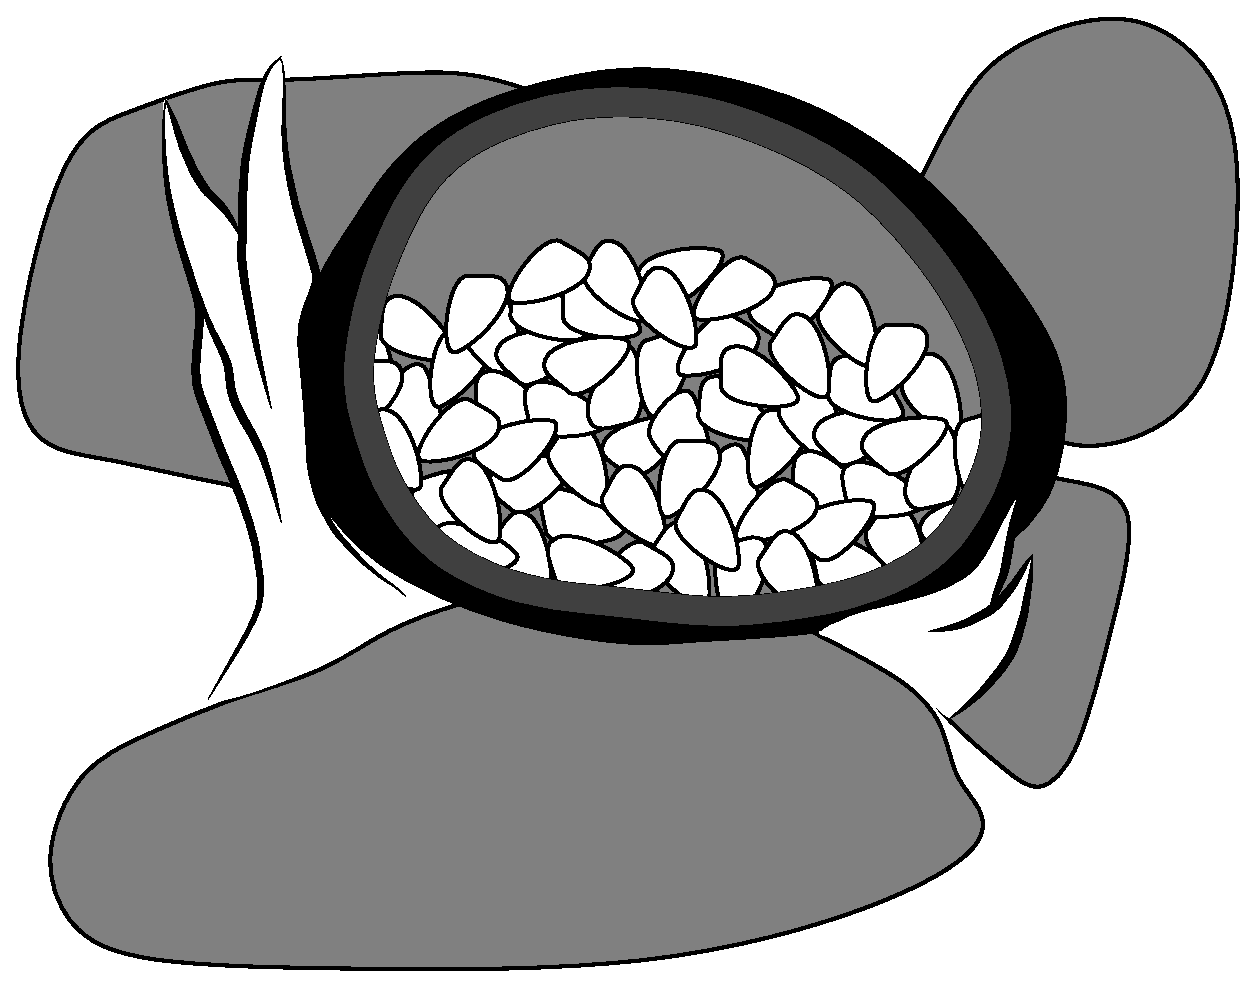
\includegraphics[width=0.47\textwidth]{cancha.eps}
  \end{center}
  \vspace{-20pt}
  %\caption{Zandor}
\end{wrapfigure}
Mi familia no era rica, y talvez ese concepto escapaba de mi entendimiento en aquella época, mas, nada de lo que realmente me importaba me faltaba.   
Yo recuerdo que mi casa era de adobe y madera, con techo de tejas; mi mamá cocinaba sobre una pequeña fogata, y mis hermanas y yo, ciertamente, usábamos con mucha frecuencia ropa que, a simple vista, cualquier persona consideraría que eran varias medidas menores de las que precisábamos;
sin embargo, para mí, mi casa era un castillo amplio y fresco, al cual yo iba a descansar después de volver de la escuela o del trabajo en la chacra.
La cocina de mi mamá era la mejor, llena de sabores obtenidos de los mismos productos que cultivábamos ou cuidábamos; en días especiales mi papá iba al río y comíamos pescado, otras veces, en la época de la seca, comíamos charqui, y más comúnmente alguna mezcla de huevos de perdiz o de gallina, dependiendo de la suerte del día.
En nuestras comidas no podían faltar en el queso y la leche, que tanto podían ser de cabra o de vaca.
Los postres dependían de la estación del año, pues las frutas como tunas, duraznos, higos, pepinos dulces, sanky entre otras, tenían su temporada. También habían épocas para sobremesas elaboradas con maíz fresco y otras con calabaza, con esta última mi mamá hacía mi mazamorra favorita; era increíble para mí que una crema de semejante majestad podía ser construida con apenas un poco de azúcar, canela, clavo de olor y calabaza.

A mis hermanas y a mí nos gustaba jugar juntos, salir a pasear buscando frutas o ir a apreciar animales silvestres; e, en general, no teníamos discusiones importantes, sin embargo, debo reconocer que, de cuando en cuando, yo acostumbraba hacer alguna maldad.
En esos casos, ellas abrían una reclamación con las máximas autoridades de la casa, con los señores que gobernaban y decidían sobre el bien y el mal, es decir, mis padres. 
recuerdo que al principio mi papá me hablaba con frases como -- Aurelio, no debes esconder la muñeca de tu hermana --- si el asunto era más grave el me decía --- Aule! Por qué colocaste un grillo en la cabeza de tu hermana? --- y si mi insistencia en la búsqueda de problemas llegaba a niveles peligrosos para mi existencia, mi papá me decía --- Aulicha! Por qué colocaste ají en el caramelo de tu hermana? ---
Así, cuando yo escuchaba que mi papá me llamaba Aulicha, yo ya sabía que mi suerte había sido decidida y que una chicoteada estaba próxima. La idea de huir siempre pasaba por mi cabeza, mas mis experiencias anteriores me indicaban que eso solamente iba a perjudicarme más, e iba resignado delante de mi papá, inclusive, en varias ocasiones, el me pedía que lleve ese chicote de tres puntas, pequeño y veloz, que era al mismo tiempo, un viejo conocido y mi principal antagonista. 

Mi vida en el campo siempre estaba llena de contrapuntos, tantos eran los momentos tristes cuanto los alegres, y  algunas veces, mas de las que me permitirían pensar que era solo una casualidad, los momentos tristes preparaban un camino inevitable e irreversible a épocas alegres, y viceversa; como un ciclo que se retro-alimenta para mantenerse perpetuo.
Así, una de mi mayores alegrías era cuando mi papá retornaba de viaje, generalmente de la costa del Perú, no solo debido a la tristeza y la añoranza que dejaba su partida y la alegría que traía su retorno, sino también porque el volvía lleno de regalos. 
El nos traía dulces, galletas, juguetes, ropas y artículos diversos; los cuales, comúnmente, nosotros en la sierra no teníamos acceso.
Por otro lado, entre mis momentos mas tristes, estaba la perdida de algún ser querido y la consecuente impotencia al no ser capaz de evitar su partida.
No obstante, todo eso es parte de la vida, y me gustaría compartir con ustedes algunos de esos momentos.





%Ayacucho é uma cidade do distrito de Ayacucho, na província de Huamanga, no departamento de Ayacucho, no Peru



%----------------------------------------------------------------------------------------
%	BOOK PART
%----------------------------------------------------------------------------------------


\partimage[0.3]{yingyang-dog-gray.eps}
\part{A dualidade do ser}



%----------------------------------------------------------------------------------------
%	CHAPTER ONE
%----------------------------------------------------------------------------------------

\chapter{Zorra}
Quando era criança, minha família tinha uma cadela que se chamava Zorra, ela era de caráter gentil; meu pai e eu costumávamos ir com ela a todos os lados. Em ocasiões em que pelos caminhos nós avistávamos a algum conhecido ou familiar, eles gritavam --- bom dia Don-Juande! --- E nós respondíamos suas saudações com a mesma alegria e energia.
Meu pai, na verdade, se chamava Juan de Dios (João de Deus); porém, carinhosamente, todo mundo preferia chamar a ele Don-Juande.

Eu provavelmente teria seis anos nessa época, e lembro de forma clara como minha cadela ia correndo de forma ágil adiante de nós, abrindo-nos caminho por meio dos montes, ladrando e sorrindo.
Estas caminhadas eram muito comuns, pois tínhamos que ir a levar comida a nossa vaca, a procurar ela quando se perdia, ou a dar manutenção à chacra.
Num princípio, eu não tinha percebido que minha cadela tinha algumas más costumes, pois com ela nós convivíamos e andávamos de dia, e seu comportamento era irrepreensível. 

Ainda lembro a primeira vez que fui ao rio, acompanhando a Zorra e a meu pai; pois minha mãe tinha encarregado a ele, com caráter de urgência, obter alguns peixes para serem fritos no almoço; eu rapidamente me uni a tão nobre encomenda, pois gostava de sair a andar. 
Para chegar ao rio tivemos que descer uma ladeira com um caminho cercado de plantas de figo das índias; quando chegamos eu vi que as margens das águas estavam cheias de juncos, sendo esse um lugar ótimo para explorar e brincar; assim, enquanto meu pai pescava, eu e minha cadela procurávamos ninhos com ovos de perdiz; porem, Zorra sempre os achava primeiro, comia tudo, ou quase tudo, e eu só podia salvar alguns para mim.


Dessa forma passaram alguns anos, onde ninguém chegou a casa trazendo alguma reclamação ou comentário sobre ela; porém, um dia entrei na minha horta e  fiquei surpreso ao achar varias coisas dentro de um esconderilho. Havia uma sacola de tecido com pão, outra com açúcar, algumas com doces, ferramentas pequenas espalhadas, etc. 
Para mim tudo isso era inacreditável, pois nós só tínhamos coisas como açúcar ou bolachas, quando meu pai voltava de suas viagens após trabalhar quatro meses em Ica, ou alguma outra cidade grande.
Num primeiro momento, a alegria invadiu meu coração, mas lembrei que meu pai era uma pessoa muito rigorosa, não gostava pegar as coisas dos outros, e dizia --- se você encontra alguma coisa no caminho, no campo, ou na pampa, você não deve pegar ---, e ele agregava, --- seguramente alguém deixou cair, a pessoa que perdeu vai voltar a procurar, e se você leva, ela não vai encontrar ---, 
eu lembrava muito bem desse ensinamento, pois uma vez quando estava na solidão do campo, pastando a minha vaca, achei uma ferramenta para fazer fios de lã, que no meu povo chamávamos de callapa; provavelmente a ferramenta era de algum outro pastor que passou por ali, mas nesse momento não pensei nisso, só peguei ela e me dirigi a minha casa; já na tarde, cheguei  muito contente, falando --- Mamãe, papai, olha o que achei no campo! --- 
Meu pai imediatamente respondeu: --- Aqui não tem nada para ser encontrado! Isso é de alguém, alguma pessoa perdeu e vá ir a procurar, anda e deixa isso no lugar que você achou ---. 
Nesse momento, um frio desceu desde a ponta da minha cabeça até as pontas dos meus pés, pois já eram quase as seis da tarde, todo estava obscuro, as poucas luzes eram muito distantes e chegavam das casas dos vizinhos, --- pois la no povo, as famílias moravam em casas que estavam separadas, uma da outra, por uma grande distância, 200, 300, 400 metros e algumas vezes até mais  ---, e para finalizar, eu era muito medroso no que se refere a lugares obscuros e a onde tinha que ir estava muito longe.

Diante da ordem do meu pai, eu fui correndo e chorando nessa direção, no caminho, não podia distinguir as coisas a uns metros de mim, pois não tínhamos lua essa noite; porém, quando estava quase na metade do meu destino e meu caminhar era cada vez mais hesitante, observei a meu redor, e numa trilha paralela à minha, entre pedras e árvores grandes, vi a meu pai me seguindo a escondidas e a uma distância significativa.
Com essa certeza no meu coração eu segui meu caminho com um pouco mais de tranquilidade, pois sentia que meu pai estava me cuidando; mesmo assim, eu seguia chorando, pois, na serra a noite é absoluta e densa, e os sons do caminho alimentavam facilmente a imaginação de uma criança.
No último terço do caminho eu decidi ir correndo, pois, sentia que já não podia aguentar mais tempo essa situação; por fim cheguei a meu destino e deixei a callapa lá.
Na volta também senti a presença do meu pai uns metros atrás de mim, ou pelo menos isso queria acreditar eu, e cheguei a minha casa em menos tempo do que gastei para ir, e quando entrei, meu pai estava sentado lá, como se nada houvesse acontecido.


Por essa velha experiência, e tendo a certeza da autoria de zorra, pois esse esconderilho era um dos seus lugares favoritos, eu tive muito medo por ela; pois sabia que meu pai não ia gostar que Zorra estivesse pegando as coisas de outras pessoas; pelo que se avisava a meu pai, ele iria castigar ela severamente; por esse motivo decidi não falar nada sobre minha descoberta, porém, tenho que reconhecer que, além do amor a minha cadela, também pesou na minha decisão que o lugar estivesse cheio de açúcar, pão e outras coisas, que para nós, gente da serra, eram luxos. 
Por esse motivo, eu iniciei a passar por ali antes de ir à escola ou a chacra, para comer bolachas, água com açúcar, ou qualquer outra coisa boa que estivesse por ali. 
Para meu desespero, um dia Zorra trouxe demasiadas coisas, não sei de onde pegou elas, pois, ela só trabalhava de noite, enquanto as pessoas da casa dormiam. Assim, diante desse aumento na criminalidade que desbordava seu esconderilho, meu pai descobre a situação.
Muito para meu pesar, ele castigou severamente a Zorra, desde minha casa eu só escutei seus lamentos recebendo a punição, pois eu preferi não ver.
Depois dessa vez, ela deixou de  levar as coisas à horta, e o problema parecia resolvido, porém, logo descobriríamos que longe da casa, numa pedra grande e obscura, perto da casa de um vizinho, Zorra havia reiniciado suas atividades; assim, de dia, diante os olhos da família, se comportava com uma cadela exemplar, porém de noite roubava as mais variadas coisas dos vizinhos.

Nesse momento foi a primeira vez que uma pessoa chegou a minha casa a fazer uma reclamação, o pagante denunciou que ele tinha visto em pessoa como Zorra havia entrado na sua casa a roubar, a indignação do meu pai foi tão grande quanto sua vergonha, pois não foi um vizinho familiar nosso, que poderia entender a situação, se não que foi uma vítima que morava muito longe de nós, em outro povo, que foi perguntando entre os vizinhos até achar suas coisas e logo nossa casa.
Nessa ocasião meu pai castigou mais duramente a Zorra; diante dessa difícil situação, minha maior tristeza era que eu já compreendia que esse problema não ia a solucionar-se com outro castigo, e minhas dúvidas foram confirmadas quando percebi que ela seguia saindo de noite. 
Muito tempo depois descobriríamos que Zorra novamente tinha mudado de esconderilho, e que levava suas coisas em outra pedra grande, na casa de uma vizinha que era viúva e que carinhosamente chamávamos avó Mesla; --- na verdade, ela não era familiar nosso, mas a costume na serra era chamar avó a qualquer pessoa de idade, como sinal de respeito, pois vivemos com eles como se fossem nossa família ---.
Assim, antes que alguma pessoa da minha casa conhece-se esse novo lugar, onde Zorra ocultava seus objetos roubados, outra pessoa chegou a denunciar novamente à cadela; e mesmo que meu pai castigou, gritou e tentou seguir ela, não conseguimos achar onde ela escondia as coisas; assim, o tempo transcorreu sem que essa incógnita fosse resolvida. 

Um dia, meu pai, meus irmãos e eu decidimos descer ao rio para pescar, porém, esse dia não achamos a Zorra para que nos acompanhe, quando chegou a hora das quatro ou cinco da tarde, quando estávamos prontos a regressar a casa com a pesca do dia, escutei um ruído entre os juncos do rio, onde costumava brincar com Zorra, por pura curiosidade me acerquei a averiguar que era esse ruido como um choro agudo; para minha surpresa era um cachorrinho, pequeno e pretinho, que minha cadela havia parido.  
Para que meu pai não veja ele, eu escondi o filhote dentro do meu agasalho, pois desconfiava que ele me deixa-se levar um novo cachorro a casa, dado que os problemas que Zorra gerava já eram suficientes para nós, como para arriscar mais a reputação da família com outro cachorro.

Só quando cheguei a casa tireo o cachorro de dentro das minhas roupas, e diante dos meus irmãos, minha mãe e meu pai, presentei o novo membro da família. Como nessa época, minhas irmãs estavam aprendendo a ler usando um livro chamado "Lola e Pepe", onde nas suas histórias descreviam a um cachorro chamado Zandor, eu decidi usar esse nome para meu novo cachorro. 
Mesmo com seus novos deveres de mãe, Zorra não deixava de causar problemas, pois a nossos ouvidos chegavam histórias de roubos em povos distantes, e as ausências de Zorra se volviam cada vez mais prolongadas.
Para nossa má sorte, num povo vizinho, se tinha espalhado a notícia que era uma cadela a responsável de todos os roubos, e num triste dia, as pessoas se organizaram, conseguiram encurralar e atrapar ela, e finalmente, deram morte a minha querida Zorra.
Esse mesmo dia chegou a minha casa a notícia da sua morte, entre lágrimas e lamentos fomos a esse povo para enterrar a nossa cadela, pois nos informaram que eles simplesmente tinham jogado seu corpo na beira do rio; quando chegamos lá, choramos até que nossas lágrimas se secaram, pois, ela tinha sido nossa amiga fiel, e mesmo que soubéssemos das suas más costumes, nós amávamos ela.
Nesse mesmo lugar, ao finalizar o dia e com o rio como testemunha, fizemos uma pequena cerimônia, e enterramos a quem em vida foi conhecida por nós como Zorra.

Ao dia seguinte, a notícia tinha se espalhado no meu povo, e mesmo que nós assumimos que não receberíamos nenhuma condolência de parte dos vizinhos, a avó Mesla chegou à porta de nossa casa chorando, e entre seus lamentos dizia:
\begin{quotation}
Eu não tinha panela, e Zorra me levou uma panela; 
eu não tinha frigideira, e Zorra me levou uma frigideira; 
eu não tinha colher, e Zorra me levou uma colher;
eu não tinha faca, e Zorra me levou uma faca;
quando tive fome, Zorra me levou pão ...  
\end{quotation}
Minha mãe abraçava ela, enquanto avó Mesla continuava com sua litania, por aquele animal que, a seu modo de ver, só tinha chegado a sua vida para ajudar ela no seu momento de maior necessidade.
 



%----------------------------------------------------------------------------------------
%	CHAPTER TWO
%----------------------------------------------------------------------------------------

\cleardoublepage
\newpage
\ifdefined\EnableIncludeImages
    \ThisULCornerWallPaper{1.0}{chapterimage.eps}
\fi
\chapter{Zandor}

Após a morte de Zorra, toda a família ficou muito triste, pois apesar de seus maus costumes, ela sempre foi muito amorosa conosco; por isso, sentíamos sua falta como se fosse um membro da família. 
Assim, passamos muito tempo chorando, sobretudo minhas irmãs e eu, que ainda éramos crianças. 
Muitas vezes vi a Teodosia ---  minha irmã mais velha, a qual carinhosamente chamávamos ``Tulaco'' ---, iniciar a chorar em silêncio ao ver o lugar onde Zorra dormia; inclusive Diofelia  --- ``Dio'', a minha irmã mais nova ---, apesar de sua curta idade, já sabia distinguir a morte e a ausência que ela deixa. 
Eu também chorava, talvez mais do que elas, porque Zorra era minha companheira fiel, ela me seguia em todos os lugares onde eu ia; pois, ao ser o filho homem da casa, eu era quem tinha que sair para trabalhar na chacra com meu pai, e Zorra sempre fazia mais alegres e memoráveis esses momentos.
Nosso único conforto era que tínhamos o Zandor; nós o amávamos por ser o último presente que Zorra nos deixou.
Eu olhava para Zandor --- todo pequeno e pretinho --- e ficava maravilhado com o quanto era fofo. Sua presença me dizia que, de alguma forma, uma parte de Zorra ainda estava conosco. 
Assim, Zandor cresceu sendo criado com muito cuidado e carinho por todos nós;
entretanto, a personalidade de Zandor era completamente distinta da de sua mãe; ele era um cachorro muito honesto e era evidente para nós que ele não tinha nenhuma dos maus costumes de Zorra. 
\ifdefined\EnableIncludeImages
\begin{wrapfigure}{r}{0.45\textwidth}
  \begin{center}
  \vspace{-20pt}
    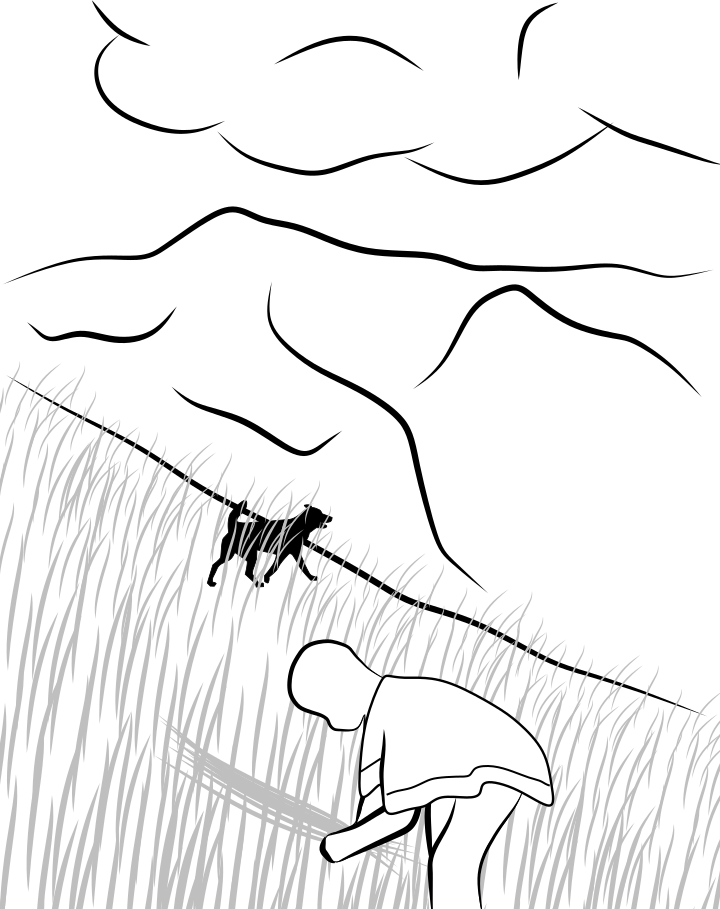
\includegraphics[width=0.43\textwidth]{pasto-zandor-aulicha}
  \end{center}
  \vspace{-20pt}
  %\caption{Figo das índias.}
\end{wrapfigure}
\fi
Desde pequeno eu levava Zandor a todas as minhas caminhadas pelo campo; como minha família tinha vacas, eu tinha que ir dar-lhes comida e atendê-las, e comumente recompensava Zandor por sua companhia dando-lhe leite fresco, que eu mesmo ordenhava para matar a nossa fome. 
Com todos esses cuidados, em pouco tempo Zandor virou um cachorrinho forte e muito brincalhão.
Ele me ajudava a cuidar das vacas e assustava os pássaros que vinham comer as sementes na chacra. Quando eu gritava seu nome, ele vinha correndo e se parava de frente a mim com a severidade de um soldado diante do seu general; ele era tão inteligente quanto uma pessoa e bem mais obediente que eu mesmo.

Um dia, quando estava no campo com Zandor, observamos que uma perdiz saía voando de uns arbustos. Para Zandor, que ainda era filhote, foi a primeira vez que ele viu uma perdiz; eu, pelo contrário, já tinha experiência com essas aves e sabia que próximo a esse lugar acharíamos um ninho, ovos ou crias. 
Automaticamente, gritei:\\\indent
--- Zandor! Vamos buscar ovos!\\\indent
Ele latiu ao sentir minha empolgação e avançou junto a mim na direção que eu indiquei para ele. 
Era gostoso ver Zandor, pequeno, porém corajoso, batendo seu rabinho, cheirando para todos os lados, levantando e recolhendo suas orelhas; como se, naquela primeira missão de busca, quisesse demonstrar sua eficácia usando ao máximo todos seus sentidos. 
Só procuramos uns minutos e de repente os vimos\\\indent
--- Olha Zandor! Ovos! --- gritei.\\\indent
Ele latiu como afirmando minha exclamação, e me acerquei ao ninho para recolher todos os ovos. Zandor não pegou nenhum, ele só me olhava contente enquanto eu os colocava num saquinho de tecido para protegê-los e levá-los a casa. 


Esse procedimento se tornou comum, e cada vez que eu saía para procurar as nossas vacas, também aproveitava para procurar ovos de perdiz com Zandor; quando os achávamos, eu os levava muito contente para minha mãe; de modo que, todos os dias, nós voltávamos com 8, 12 ou até 15 ovos. 
Com o passar dos meses, Zandor virou um especialista em encontrar ovos, pois ele já não era um filhote, e eu não precisava acompanhá-lo mais. Assim, enquanto eu trabalhava, ele saía por conta própria a procurar ovos; no instante em que ele os achava, latia repetidas vezes e sem descanso, até chamar minha atenção, de modo que minha única missão era recolhê-los e levá-los para casa.
\ifdefined\EnableIncludeImages
\begin{wrapfigure}{r}{0.43\textwidth}
  \begin{center}
  \vspace{-20pt}
    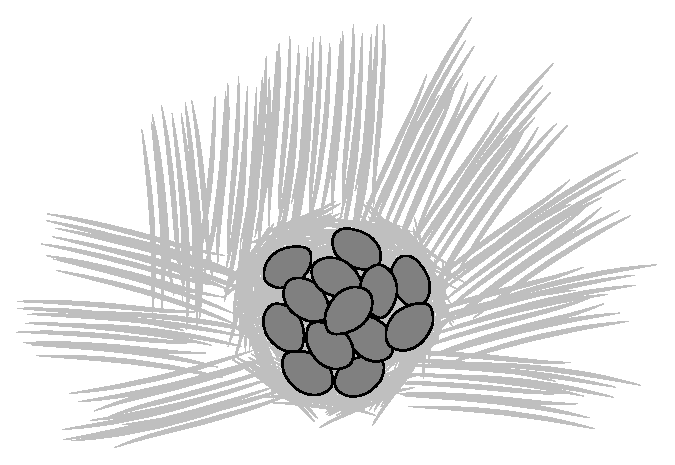
\includegraphics[width=0.40\textwidth]{huevos.eps}
  \end{center}
  \vspace{-20pt}
  %\caption{Figo das índias.}
\end{wrapfigure}
\fi
Algumas vezes, cozinhávamos os ovos, outras vezes os fritávamos; e numa dessas ocasiões, meu pai chegou em casa quando estávamos cozinhando-os,\\\indent
--- e esses ovos?--- perguntou ele, 
e eu, contente e cheio de orgulho, respondi:\\\indent 
--- Zandor achou!\\\indent
Ele meditou um pouco e replicou:\\\indent 
--- Zandor achou... e que coisa deram a ele?\\\indent
A pergunta me pegou de surpresa e falei em voz baixa:\\\indent 
--- Nada pai, só a comida da casa... \\\indent
Meu pai me olhou e falou calmamente: \\\indent
--- Se foi ele quem achou, ele também deve participar.\\\indent
Nesse momento meu pai pegou um ovo cru e deu para o cachorro, Zandor pegou contente o ovo e lambeu até sobrar só a casca. A partir de então, Zandor se acostumou a comê-los sempre que lhe ofereciam. 
Assim, cada vez que ele encontrava ovos, eu os levava para casa, os entregava a minha mãe e ela por sua vez entregava dois a Zandor; porém, nunca lhe dávamos os ovos quando ele os encontrava, somente na casa, ele por sua parte sabia esperar e nunca pegou nenhum, só esperava pacientemente o momento que minha mãe entregasse a ele seus ovos e ia contente a seu cantinho para comê-los.


Para mim, Zandor era maravilhoso, em qualquer lugar aonde eu ia, ele me acompanhava, quando estava triste ele se sentava a meu lado e até chorava comigo fazendo um som agudo, que eu sentia cheio de solidariedade. 
Por outro lado, se ele percebia que eu estava contente, levantava suas orelhinhas e iniciava a pular e correr de um lado a outro. Assim, durante muito tempo, andamos e crescemos juntos... o tempo passou e eu completei oito anos, e logo, nove anos de idade.

Um dia meu pai decidiu abater um boi; lá na serra não se mata um boi sem nenhum motivo, só em ocasiões importantes como festas regionais, casamentos ou eventos semelhantes. No entanto, eu sabia que nessa época não tínhamos nenhuma festividade e pensava que a meu pai simplesmente ocorreu-lhe abater o boi sem nenhum motivo, mas não era assim. 
Eu tinha um irmão mais velho que morava na capital, em Lima; eu não o conhecia, só sabia de sua existência, pois meus pais sempre falavam sobre sua vida lá e se referiam a ele como ``Seve''; nessa época, eu pensava que ele se chamava dessa forma, não obstante, esse não era seu nome e, sim, Severino. Eu não o conhecia porque viajou para Lima quando eu era muito pequeno, seguramente o vi nessa época, mas eu não tinha lembrança alguma. 
Assim, meu pai e minha mãe tinham a intenção de fazer charque para mandar-lhe como encomenda; com essa finalidade, decidiram abater o boi e prepararam cuidadosamente sua carne com muito sal.

\ifdefined\EnableIncludeImages
\begin{wrapfigure}{r}{0.49\textwidth}
  \begin{center}
  \vspace{-20pt}
    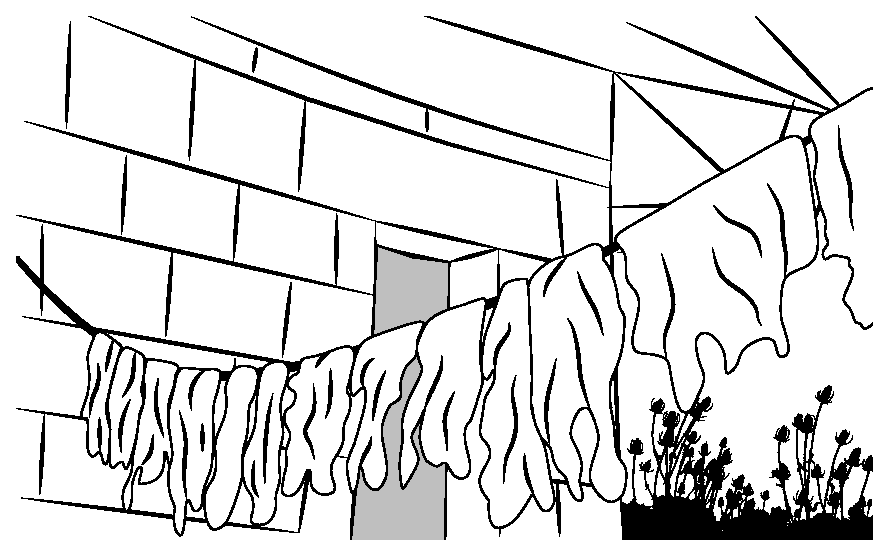
\includegraphics[width=0.47\textwidth]{charque.eps}
  \end{center}
  \vspace{-20pt}
  %\caption{Zandor}
\end{wrapfigure}
\fi
Nosso lar estava composto por uma casa pequena e uma grande, ambas separadas por vários metros entre si; nossa família morava na casa grande e usávamos a pequena para guardar ferramentas, grãos e, em geral, alimentos não perecíveis. 
Perto da casa pequena, nós tínhamos duas figueiras; nesse dia meu pai usou uma delas para amarrar uma corda até a casa pequena, e sobre ela pendurou a carne para secar com o sol; porém, ele decidiu pendurar uma perna de boi no tronco da outra figueira, pois essa peça de carne pesava muito.
Lá o costume é recolher a carne e levá-la para a casa durante a noite, para que os animais de hábitos noturnos não viessem para comê-la, de modo que no dia seguinte, pela manhã, com os primeiros raios do sol, a carne era novamente pendurada; não obstante, nesse dia meu pai recolheu só o charque que estava pendurado na corda e esqueceu a perna que tinha colocado na outra figueira. 
O pior foi que ali, onde meu pai deixou a carne, tranquilamente qualquer cachorro, zorro, ou outro animal carnívoro da serra, poderia pegá-la facilmente, sem a necessidade de pular, uma vez que não estava a muita altura.

Essa noite Zandor não parou de latir; nós, na casa grande, só escutávamos seu barulho com curiosidade, dado que nenhum membro da família lembrou da perna pendurada na figueira. 
Pelo barulho, só reconhecíamos que algumas vezes chegavam outros cachorros, outras vezes não escutávamos nenhum outro animal, só o Zandor latindo com muita raiva e força; meu pai, bravo pelo ruído, só falava:\\\indent
--- Que coisa quer esse cachorro que não nos deixa dormir!\\\indent
Porém, ele não saía da casa grande para indagar sobre a situação. 
Eu tinha muito medo por tudo o que estava acontecendo; pois, na serra, contam histórias dos seres que habitam a noite. 
Alguns diziam que à noite anda o ``cuco''\footnote{Também chamado coca ou coco, este é um ser mítico, uma espécie de fantasma, bruxa ou bicho-papão que anda de noite pelos caminhos.}, e as crianças tinham um terror extremo a esse ser; para piorar a situação, meu pai tinha o costume de contar-nos histórias sobre suas viagens, de como à noite achou o ``cuco'' nos caminhos da serra, ou também que, em algum povoado perto, o ``cuco'' tinha matado algum vizinho, que tinha chupado o sangue de outro ou simplesmente assustado algum caminhante noturno. Devo reconhecer que apesar do terror que me causavam as histórias do meu pai, eu gostava de conhecê-las e passar medo ouvindo-as; ele sempre me contava suas aventuras de quando saía para trabalhar em outras cidades e das coisas que viu, dos problemas que aconteciam no caminho e dos personagens que apareciam quando ele se deslocava a pé.

\ifdefined\EnableIncludeImages
\begin{wrapfigure}{r}{0.49\textwidth}
  \begin{center}
  \vspace{-20pt}
    \includegraphics[width=0.47\textwidth]{AgriornisSolitariaSmit.jpg}
  \end{center}
  \vspace{-20pt}
  %\caption{Zandor}
\end{wrapfigure}
\fi
Por exemplo, um dia meu pai me contou que quando estava viajando, caminhando desde nosso povo até ``Cangallo'', um povoado distante, no meio do caminho, a noite chegou, e ele iniciou a procurar entre os trilhos alguma casa que pudesse dar-lhe pousada. Enquanto ele estava nessa tarefa, escutou um pássaro ao qual nós na serra chamamos ``huaychao''\footnote{Também escrito como waychaw, esta é uma palavra quéchua que significa: avisar, anunciar, advertir ou notificar. ``Huaychao'' é uma onomatopeia do som que faz a ave cujo nome científico é Agriornis montanus.}, cujo canto é de mau augúrio.
Meu pai falava que quando o ``Huaychao'' canta, é porque o mal está perto, que ele canta porque viu o mal andando, talvez na forma de algum ``jarjacha''\footnote{Também chamado carcaq ou qarqacha.}. 
Para nós, os ``jarjachas'' são seres da noite, são pessoas que se levantam dos seus túmulos, pois ao terem feito coisas terríveis em vida, estão condenadas a não morrer e vagar de noite entre o sofrimento e a ira. 
Então, meu pai sempre me advertia muito sério que, se na noite escutava ao huaychao, devia ter muito cuidado porque seguramente um ``jarjacha'' estava perto. 
Na sequência dos fatos, quando meu pai escutou ao huaychao, começou a correr pulando pedras e atravessando riachos até que, só e assustado, achou uma casa; rapidamente bateu à porta e de dentro, escutou uma voz de mulher que lhe perguntava:\\\indent
--- Boa noite! Quem está aí?\\\indent
Meu pai, todo assustado, tentou lhe explicar que era só um viajante, que a noite tinha chegado na metade do seu caminho e que somente precisava de um lugar para dormir. A senhora, do interior da casa, respondeu-lhe que, da mesma forma que ele falou, seres que não são pessoas, ``cucos'', andam pela noite enganando os moradores para conseguir entrar em suas casas,\\\indent
--- de repente você é um deles! --- Disse a senhora e negou a meu pai um lugar para dormir.\\\indent
Ele insistiu com a voz tremida pelo medo, porque sabia que tudo isso era verdade, pois ele já tinha escutado ao huaychao e sabia que o mal estava perto. Por fim, após discutir muito, a senhora se comoveu e deixou a meu pai entrar em casa. 
A senhora, toda curiosa pela situação, perguntou a meu pai por que andava à noite, e ele explicou que só estava tentando ir de Occo até Cangalho; porém, teve problemas no caminho e a noite lhe pegou. 
Imediatamente a senhora respondeu em tom maternal:\\\indent 
--- Por que você anda à noite? Só ontem um ``jarjacha'' comeu uma pessoa, agora esse vizinho está morto, hoje mesmo enterramos ele.\\\indent
Por todas essas histórias, sair da casa grande de noite, só porque o cachorro latia, era uma completa temeridade; até meu pai tinha medo de sair, ele só gritava para Zandor de dentro da casa, segurando sua ``guaraca''\footnote{Corda muito versátil que pode ser usada como cinto de calças ou para disciplinar crianças desobedientes.}, golpeando com ela a parede. 
Os demais membros da família, incluindo-me, só escutávamos resignados, tentando dormir apesar do barulho.

Assim, a noite passou, e praticamente nenhum de nós conseguiu dormir. 
Quando os primeiros raios do sol tocaram a nossa janela, todos nós saímos em direção à casa pequena e, para nossa surpresa, vimos a perna de boi pendurada na figueira. 
Para nós foi evidente que, durante a noite, os animais do campo tinham chegado para comer a carne e Zandor tinha defendido-a, brigando, latindo e sem dormir.
\ifdefined\EnableIncludeImages 
\begin{wrapfigure}{r}{0.47\textwidth}
  \begin{center}
  \vspace{-0.5cm}
    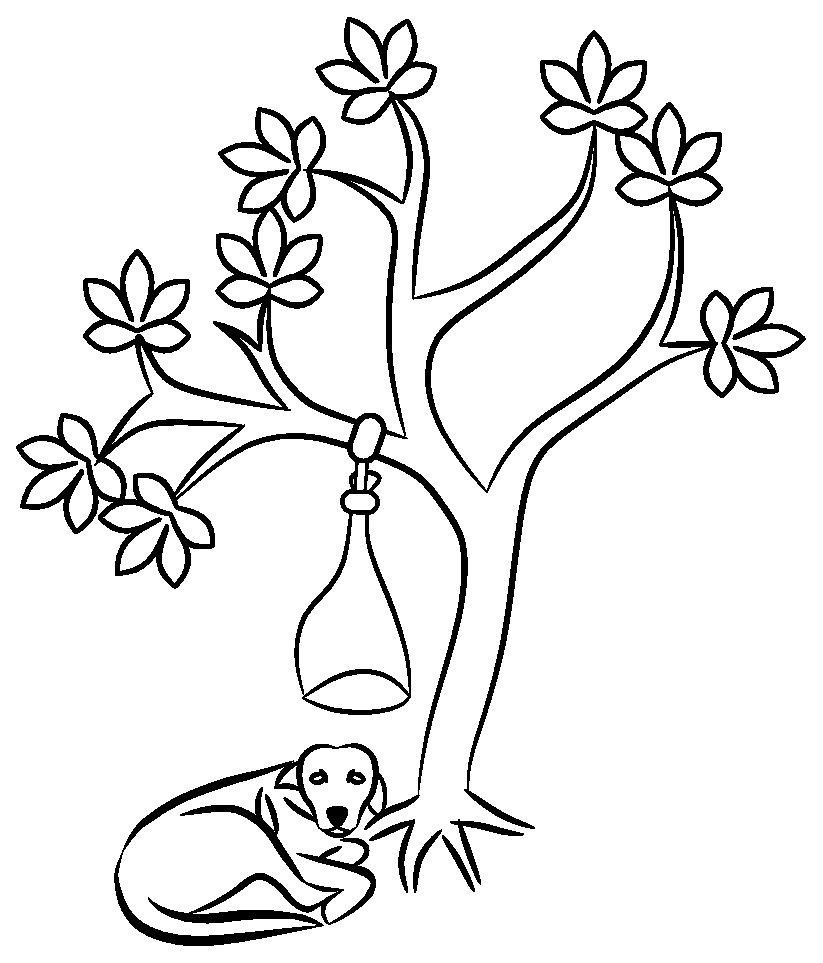
\includegraphics[width=0.45\textwidth]{perro-fiel-1.eps}
  \end{center}
  \vspace{-0.5cm}
  %\caption{Zandor}
\end{wrapfigure}
\fi
Ele estava aconchegado, encolhido em forma de bolinha abaixo da perna de boi e, ao nos ver chegar, só nos dirigiu um olhar cansado enquanto abanava o rabinho. Meu pai se admirou pelo desempenho de Zandor, pois a carne estava intacta.\\\indent
--- Como me esqueci da perna! Por isso chegavam os cachorros! --- exclamou meu pai.\\\indent
Automaticamente entrou na casa, pegou uma faca, cortou um pedaço grande de carne da perna de boi, ainda pendurada na figueira, e a entregou a Zandor como um prêmio; só nesse momento, ele olhou a carne com vontade, pegou seu prêmio e foi para o canto dele para comer.

Assim, Zandor cresceu sendo sempre um cachorro honrado. Se você não dava alguma coisa, ele não pegava; por isso, toda a família o respeitava. Além disso, no campo, os cachorros sempre são bem cuidados; eles comem a mesma comida dos donos de casa e são tratados com carinho, sendo eles considerados como membros da família.



%----------------------------------------------------------------------------------------


%----------------------------------------------------------------------------------------
\backmatter
\chapterwithtocfalse

%----------------------------------------------------------------------------------------
%	COLOFÃO
%----------------------------------------------------------------------------------------
\cleardoublepage

\null
\vfill

\begin{flushright}
{\normalsize \it Continuará.
\vspace*{4pt}}
\end{flushright}

\newpage

\null
\vfill
\thispagestyle{empty}


{\normalsize \it Este libro fue producido por \myauthor, editado y diagramado usando \LaTeX,
con un tipo de fuente \showfont,
para ser impreso en un papel tamaño \imprimirpapersize. Edición creada en \imprimirdata.
\vspace*{4pt}}







%----------------------------------------------------------------------------------------

\end{document}
